
%(BEGIN_QUESTION)
% Copyright 2006, Tony R. Kuphaldt, released under the Creative Commons Attribution License (v 1.0)
% This means you may do almost anything with this work of mine, so long as you give me proper credit

The following storage vessel holds a liquid with a density of 60 lb/ft$^{3}$.  The $\Delta$P transmitter is located 5 feet above the bottom of the vessel and has a remote seal with capillary tubing whose fill fluid has a specific gravity of 1.9.  The desired level measurement range is 0 feet to 11 feet:

$$\includegraphics[width=15.5cm]{i00261x01.eps}$$

Assuming an electronic transmitter with an output range of 4 to 20 mA, and a calibration accuracy of $\pm$ 0.2\% of span, complete the following calibration table for the transmitter:

% No blank lines allowed between lines of an \halign structure!
% I use comments (%) instead, so that TeX doesn't choke.

$$\vbox{\offinterlineskip
\halign{\strut
\vrule \quad\hfil # \ \hfil & 
\vrule \quad\hfil # \ \hfil & 
\vrule \quad\hfil # \ \hfil & 
\vrule \quad\hfil # \ \hfil & 
\vrule \quad\hfil # \ \hfil & 
\vrule \quad\hfil # \ \hfil \vrule \cr
\noalign{\hrule}
%
% First row
Process & Percent of & $\Delta$ pressure & Output signal & Output signal & Output signal \cr
%
% Another row
level (ft) & span (\%) & sensed ("W.C) & ideal (mA) & min. (mA) & max. (mA) \cr
%
\noalign{\hrule}
%
% Another row
  & 0 &  &  &  &  \cr
%
\noalign{\hrule}
%
% Another row
  & 10 &  &  &  &  \cr
%
\noalign{\hrule}
%
% Another row
  & 25 &  &  &  &  \cr
%
\noalign{\hrule}
%
% Another row
  & 50 &  &  &  &  \cr
%
\noalign{\hrule}
%
% Another row
  & 75 &  &  &  &  \cr
%
\noalign{\hrule}
%
% Another row
  & 90 &  &  &  &  \cr
%
\noalign{\hrule}
%
% Another row
  & 100 &  &  &  &  \cr
%
\noalign{\hrule}
} % End of \halign 
}$$ % End of \vbox

\vskip 10pt

Be sure to show all your mathematical work so that your instructor will be able to check the conceptual validity of your technique(s).  A good way to check to see if you're solving the problem correctly is to check that each and every one of your intermediate calculations (i.e. the results you get mid-way during the process to arrive at the final answer) has real physical meaning.  {\bf If you truly understand what you are doing, you will be able to identify the correct unit of measurement for every intermediate result and also be able to show where that number applies to the scenario at hand}.


\vskip 20pt \vbox{\hrule \hbox{\strut \vrule{} {\bf Suggestions for Socratic discussion} \vrule} \hrule}

\begin{itemize}
\item{} Demonstrate how to {\it estimate} numerical answers for this problem without using a calculator.
\item{} Suppose this vessel were enclosed at the top, and a remote-sealed compensating leg connected from the transmitter's ``L'' port to the top of the vessel.  How would this change the transmitter's necessary calibration?  Would it require an adjustment in zero, span, linearity, or some combination of these?
\item{} Given a 100\% full vessel, calculate the amount of pressure that would be registered by a pressure gauge connected to the bottom of the vessel.
\item{} Given a 100\% full vessel, calculate the amount of pressure that would be registered by a pressure gauge connected to the capillary tube (at the remote seal).
\item{} Given a 100\% full vessel, calculate the amount of pressure that would be registered by a pressure gauge connected to the capillary tube (at the transmitter ``H'' port).
\end{itemize}

\underbar{file i00261}
%(END_QUESTION)





%(BEGIN_ANSWER)

\noindent
{\bf Partial answer:}

% No blank lines allowed between lines of an \halign structure!
% I use comments (%) instead, so that TeX doesn't choke.

$$\vbox{\offinterlineskip
\halign{\strut
\vrule \quad\hfil # \ \hfil & 
\vrule \quad\hfil # \ \hfil & 
\vrule \quad\hfil # \ \hfil & 
\vrule \quad\hfil # \ \hfil & 
\vrule \quad\hfil # \ \hfil & 
\vrule \quad\hfil # \ \hfil \vrule \cr
\noalign{\hrule}
%
% First row
Process & Percent of & $\Delta$ pressure & Output signal & Output signal & Output signal \cr
%
% Another row
level (ft) & span (\%) & sensed ("W.C) & ideal (mA) & min. (mA) & max. (mA) \cr
%
\noalign{\hrule}
%
% Another row
  & 0 &  &  &  &  \cr
%
\noalign{\hrule}
%
% Another row
  & 10 &  &  & 5.568 &  \cr
%
\noalign{\hrule}
%
% Another row
  & 25 & $-82.28$ &  &  &  \cr
%
\noalign{\hrule}
%
% Another row
5.5  & 50 &  &  &  &  \cr
%
\noalign{\hrule}
%
% Another row
  & 75 &  & 16 &  &  \cr
%
\noalign{\hrule}
%
% Another row
  & 90 &  &  &  &  \cr
%
\noalign{\hrule}
%
% Another row
  & 100 & +12.87 &  &  &  \cr
%
\noalign{\hrule}
} % End of \halign 
}$$ % End of \vbox

%(END_ANSWER)





%(BEGIN_NOTES)

% No blank lines allowed between lines of an \halign structure!
% I use comments (%) instead, so that TeX doesn't choke.

$$\vbox{\offinterlineskip
\halign{\strut
\vrule \quad\hfil # \ \hfil & 
\vrule \quad\hfil # \ \hfil & 
\vrule \quad\hfil # \ \hfil & 
\vrule \quad\hfil # \ \hfil & 
\vrule \quad\hfil # \ \hfil & 
\vrule \quad\hfil # \ \hfil \vrule \cr
\noalign{\hrule}
%
% First row
Process & Percent of & $\Delta$ pressure & Output signal & Output signal & Output signal \cr
%
% Another row
level (ft) & span (\%) & sensed ("W.C) & ideal (mA) & min. (mA) & max. (mA) \cr
%
\noalign{\hrule}
%
% Another row
0 & 0 & $-114$ & 4 & 3.968 & 4.032 \cr
%
\noalign{\hrule}
%
% Another row
1.1 & 10 & $-101.31$ & 5.6 & 5.568 & 5.632 \cr
%
\noalign{\hrule}
%
% Another row
2.75 & 25 & $-82.28$ & 8 & 7.968 & 8.032 \cr
%
\noalign{\hrule}
%
% Another row
5.5 & 50 & $-50.57$ & 12 & 11.968 & 12.032 \cr
%
\noalign{\hrule}
%
% Another row
8.25 & 75 & $-18.85$ & 16 & 15.968 & 16.032 \cr
%
\noalign{\hrule}
%
% Another row
9.9 & 90 & +0.1795 & 18.4 & 18.368 & 18.432 \cr
%
\noalign{\hrule}
%
% Another row
11 & 100 & +12.87 & 20 & 19.968 & 20.032 \cr
%
\noalign{\hrule}
} % End of \halign 
}$$ % End of \vbox

%INDEX% Calibration: table, level transmitter
%INDEX% Measurement, level: calibration table
%INDEX% Measurement, level: hydrostatic pressure (elevated zero)

%(END_NOTES)


